\chapter{Результаты проектирования системы Интеллектуального ассистента врача щитовидной железы}

\section{Разработка микросервисной архитектуры системы}

\subsection{Паттерн API Composition}
Каждому спроектированному компоненту системы соответствует свой микросервис. Общение между микросервисами осуществляется 
синхронным и асинхронным способом. Однако в распределенных системах следует избегать лишних зависимостей между микросервисами, это
может повлеч за собой сложности в масштабировании и обслуживании системы, проблемы с каскадными ретраями, и в целом делает изолированный и
обособленные части системы зависимыми от других частей системы.\\
Для удовлетворения требовани о регистрации пользователей системы нам требуется сообщить информацию о новом пользователе в 2 компонента:
компоненту авторизации и аутентификации и компоненту управления пользователями.\\
Для избежания лишней зависимости между компонентами, мы используем паттерн Composition-API. API Composition паттерн 
— это подход в архитектуре микросервисов, который позволяет выносить логику взаимодействия между микросервисами в отдельный сервис более верхнего уровня.

\begin{figure}[H]%
	\begin{center}
		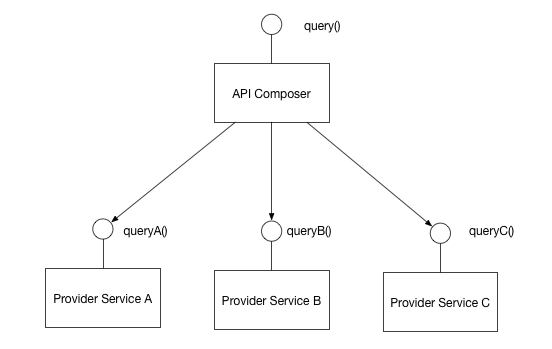
\includegraphics[width=.6\columnwidth]{./img/new/api_composition_pattern.png}%
	\end{center}
	\caption{API Composition паттерн}%
	\label{pic:api_composition_pattern}%
\end{figure}

\subsection{Способы взаимодействия между микросервисами}
Основные запросы которые будут поступать в ИИ ассистент врача, это запросы на получение того или иного ресурса. Данные запросы
реализуются посредством обычных синхронных интернет запросов, в API Composition. Далее из API Composition запросы передаются в микросервисы.


Однако стоит рассмотреть сценарий загрузки узи снимков на обработку в систему. Обработка узи снимка занимает значительное для пользователя время.
Нужен механизм, который избавит пользователя от необходимости активного ожидания результатов обработки узи снимка.\\
Решением этой проблемы - во время загрузки узи снимка, система ставит асинхронную задачу на обработку узи снимка. Если 
задача поставлена успешно, пользователь получает идентификатор задачи, после чего может посредством отдельных запросов узнать статус задачи.
В данном случае ожидание пользователя будет сведено к загрузке узи снимка.
В таком случае, схема начала обработки узи снимка будет выглядеть следующим образом:
\begin{figure}[H]%
	\begin{center}
		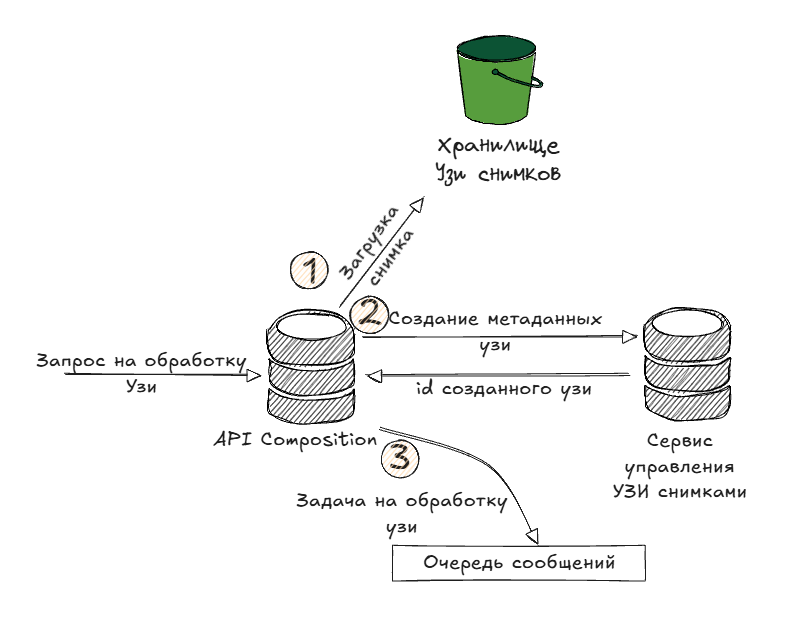
\includegraphics[width=.6\columnwidth]{./img/new/async.png}%
	\end{center}
	\caption{Схема асинхронной обработки узи снимка}%
	\label{pic:async}%
\end{figure}

\subsection{Итоговая архитектура системы Интеллектуального ассистента врача щитовидной железы}

Применяя паттерны API Composition при проектировании, а также учитывая синхронное и асинхронное взаимодействие между микросервисами,
мы получаем следующую архитектуру системы:
\begin{figure}[H]%
	\begin{center}
		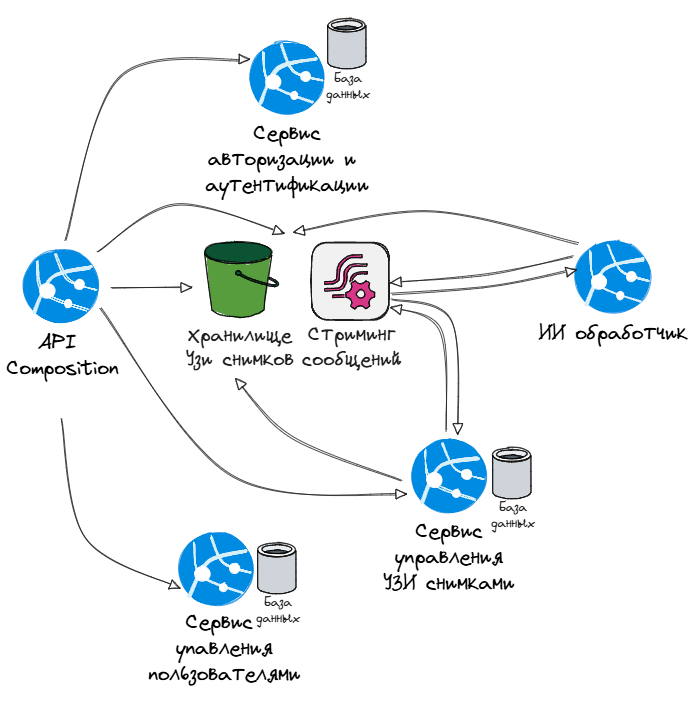
\includegraphics[width=.6\columnwidth]{./img/new/microservice_arch.png}%
	\end{center}
	\caption{Итоговая архитектура микросервисной системы}%
	\label{pic:microservice_arch}%
\end{figure}

\section{Выбор технологий и инструментов для технической реализации системы}

\subsection{Языка программирования}

\subsubsection*{Философия и дизайн языков}

\textbf{Python} следует философии простоты и читаемости кода, воплощённой в принципе \textit{"Zen of Python"}. Язык спроектирован так, чтобы код был максимально понятным и выразительным, что делает его идеальным для быстрого прототипирования и обучения программированию.

\textbf{Java} основан на принципах объектно-ориентированного программирования и философии \textit{"write once, run anywhere"}. Язык обеспечивает строгую типизацию и надёжность выполнения программ за счёт виртуальной машины Java (JVM).

\textbf{Go} создавался с целью объединить простоту синтаксиса с высокой производительностью. Разработчики Google стремились создать язык, который был бы эффективен для создания масштабируемых сетевых приложений и системного программирования.

\subsubsection*{Производительность и скорость выполнения}

По скорости выполнения языки располагаются в следующем порядке:

\begin{enumerate}
    \item \textbf{Go} --- компилируемый язык, обеспечивающий производительность, близкую к C/C++
    \item \textbf{Java} --- благодаря JIT-компиляции и оптимизациям JVM показывает высокую производительность
    \item \textbf{Python} --- интерпретируемый язык с относительно низкой скоростью выполнения
\end{enumerate}

Однако важно отметить, что Python компенсирует низкую скорость выполнения возможностью использования оптимизированных библиотек, написанных на C/C++, таких как NumPy и Pandas.

\subsubsection*{Синтаксис и удобство разработки}

\textbf{Python} обладает наиболее лаконичным и интуитивным синтаксисом. Отсутствие точек с запятой, использование отступов для обозначения блоков кода и богатая стандартная библиотека делают разработку быстрой и приятной.

\textbf{Java} требует больше \textit{boilerplate}-кода, но обеспечивает чёткую структуру и типобезопасность. Современные версии Java (начиная с Java 8) значительно упростили синтаксис благодаря лямбда-выражениям и другим нововведениям.

\textbf{Go} сочетает простоту синтаксиса с мощными возможностями. Язык имеет минималистичный дизайн, но при этом включает встроенную поддержку параллельного программирования через горутины и каналы.

\subsubsection*{Экосистема и библиотеки}

\textbf{Python} обладает самой обширной экосистемой для задач машинного обучения, науки о данных и веб-разработки. PyPI содержит сотни тысяч пакетов практически для любых задач.

\textbf{Java} имеет зрелую экосистему корпоративной разработки с такими фреймворками, как Spring, Hibernate, Apache Commons. Maven и Gradle обеспечивают надёжное управление зависимостями.

\textbf{Go} обладает растущей, но пока более ограниченной экосистемой. Встроенный пакетный менеджер и стандартная библиотека покрывают большинство базовых потребностей, особенно для сетевого и системного программирования.

\subsubsection*{Области применения}

\begin{description}
    \item[Python:] машинное обучение, анализ данных, веб-разработка (Django, Flask), автоматизация, скриптинг
    \item[Java:] корпоративные приложения, Android-разработка, веб-сервисы, большие распределённые системы
    \item[Go:] микросервисы, сетевые приложения, DevOps-инструменты, системное программирование
\end{description}

\subsubsection*{Параллельное программирование}

\textbf{Go} предоставляет наиболее элегантную модель параллельного программирования с горутинами и каналами, основанную на принципах CSP (Communicating Sequential Processes).

\textbf{Java} использует традиционную модель потоков с возможностями из пакета \texttt{java.util.concurrent}, а также современные решения вроде Project Loom.

\textbf{Python} ограничен Global Interpreter Lock (GIL), что затрудняет истинное многопоточное выполнение, хотя существуют способы обхода через multiprocessing и asyncio.


\textbf{Заключение}

Учитывая наши требования и специфику приложений, мы выбираем Golang как язык программирования для ассистента.

\subsection{Реляционные хранилища данных}
\textbf{Реляционные базы данных}: Реляционные базы данных, такие как MySQL и PostgreSQL, предлагают структурированный способ хранения данных с использованием таблиц, что позволяет легко реализовать связи между ними. Они подходят для большинства приложений, требующих согласованности и целостности данных.

\subsubsection*{Общая характеристика}

PostgreSQL и MySQL являются двумя наиболее популярными системами управления базами данных с открытым исходным кодом. Каждая из них имеет свои особенности и области применения.

\subsubsection*{Основные различия}

\textbf{Архитектура и подход}
PostgreSQL представляет собой объектно-реляционную СУБД, следующую стандартам SQL и поддерживающую сложные типы данных. MySQL изначально создавалась как быстрая и простая реляционная СУБД.

\textbf{Производительность}
MySQL традиционно показывает лучшие результаты в простых операциях чтения и веб-приложениях. PostgreSQL превосходит в сложных запросах, аналитике и операциях записи с высокой конкуренцией.

\textbf{Функциональность}
PostgreSQL предлагает расширенные возможности: поддержку JSON, массивов, пользовательских типов данных, оконных функций и процедурных языков. MySQL имеет более простой набор функций, но достаточный для большинства веб-приложений.

\subsubsection*{Области применения}

\textit{PostgreSQL} оптимален для:
\begin{itemize}
\item Сложных аналитических систем
\item Приложений с высокими требованиями к целостности данных
\item Проектов, требующих расширенной функциональности SQL
\end{itemize}

\textit{MySQL} предпочтителен для:
\begin{itemize}
\item Веб-приложений и CMS
\item Проектов с простыми запросами и высокой нагрузкой на чтение
\item Систем, где важна простота администрирования
\end{itemize}

\textbf{Заключение}

Учитывая наши требования и специфику приложений, мы выбираем PostgreSQL как основное решение для хранения данных в нашей архитектуре.

\subsection{Хранилище УЗИ снимков}

В современном мире информационных технологий выбор подходящей системы хранения данных становится критически важным решением. Каждый тип хранилища имеет свои особенности, преимущества и области применения. Рассмотрим три основных подхода к организации хранения данных.
\subsubsection*{Объектное хранилище}
Объектное хранилище представляет собой архитектуру, где данные хранятся в виде объектов в плоском пространстве имен. Каждый объект содержит сами данные, метаданные и уникальный идентификатор.
\textbf{Ключевые особенности:}
\begin{itemize}
\item Масштабируемость до петабайтов данных
\item REST API для доступа к данным
\item Отсутствие традиционной файловой иерархии
\item Встроенная репликация и обеспечение целостности данных
\end{itemize}
\textbf{Преимущества:}
\begin{itemize}
\item Практически неограниченная масштабируемость
\item Высокая надежность благодаря распределенной архитектуре
\item Экономическая эффективность для больших объемов данных
\item Идеально подходит для веб-приложений и API
\end{itemize}
\textbf{Недостатки:}
\begin{itemize}
\item Невозможность модификации объектов (только замена)
\item Более высокая латентность по сравнению с локальными системами
\item Ограниченная поддержка POSIX-операций
\end{itemize}
\textbf{Примеры использования:} Amazon S3, облачные сервисы, резервное копирование, хранение мультимедиа контента.
\subsubsection*{Файловое хранилище}
Традиционные файловые системы организуют данные в виде иерархической структуры папок и файлов. Это наиболее привычный и широко используемый подход к хранению данных.
\textbf{Ключевые особенности:}
\begin{itemize}
\item Иерархическая структура каталогов
\item Прямой доступ к файлам через файловую систему
\item Поддержка стандартных операций чтения/записи
\item Интеграция с операционными системами
\end{itemize}
\textbf{Преимущества:}
\begin{itemize}
\item Простота использования и понимания
\item Быстрый доступ к данным
\item Полная совместимость с существующими приложениями
\item Поддержка всех стандартных файловых операций
\end{itemize}
\textbf{Недостатки:}
\begin{itemize}
\item Ограниченная масштабируемость
\item Уязвимость к отказам оборудования
\item Сложность резервного копирования больших объемов данных
\item Производительность снижается при работе с миллионами файлов
\end{itemize}
\textbf{Примеры использования:} Локальные диски, NAS-системы, файловые серверы предприятий.
\subsubsection*{Распределенные файловые системы}
Распределенные файловые системы объединяют преимущества традиционного файлового хранилища с возможностями распределенной архитектуры, обеспечивая масштабируемость и отказоустойчивость.
\textbf{Ключевые особенности:}
\begin{itemize}
\item Данные распределены по множеству узлов
\item Прозрачный доступ к файлам как к локальным
\item Автоматическая репликация и восстановление
\item Горизонтальное масштабирование
\end{itemize}
\textbf{Преимущества:}
\begin{itemize}
\item Высокая доступность и отказоустойчивость
\item Масштабируемость путем добавления новых узлов
\item Сохранение привычного файлового интерфейса
\item Автоматическое распределение нагрузки
\end{itemize}
\textbf{Недостатки:}
\begin{itemize}
\item Сложность настройки и администрирования
\item Потенциальные проблемы с консистентностью данных
\item Зависимость от сетевой инфраструктуры
\item Более высокая стоимость внедрения
\end{itemize}
\textbf{Примеры использования:} Hadoop HDFS, GlusterFS, Ceph, высоконагруженные системы, big data аналитика.
\subsubsection*{Сравнительная таблица}

\begin{table}[H]
\centering
\begin{tabular}{|l|l|l|l|}
\hline
\textbf{Критерий}       & \textbf{Объектное}            & \textbf{Файловое}             & \textbf{Распределенные} \\ \hline
Масштабируемость        & Очень высокая                 & Малая                         & Высокая \\ \hline
Производительность      & Средняя                       & Высокая                       & Высокая \\ \hline
Надежность              & Очень высокая                 & Низкая                        & Высокая \\ \hline
Простота использования  & Средняя                       & Высокая                       & Низкая \\ \hline
Стоимость               & Низкая                        & Средняя                       & Высокая \\ \hline
\end{tabular}
\caption{Сравнение нереалиционных баз данных}
\end{table}

\subsubsection* {Выбор подходящего решения}
Выбор типа хранилища зависит от конкретных требований:
\textbf{Объектное хранилище} идеально для веб-приложений, резервного копирования и архивирования данных, где требуется высокая масштабируемость при умеренных требованиях к производительности.
\textbf{Файловое хранилище} остается оптимальным выбором для локальных приложений, небольших и средних объемов данных, где важна простота и производительность.
\textbf{Распределенные файловые системы} подходят для корпоративных решений с высокими требованиями к доступности и необходимостью обработки больших объемов данных с сохранением файлового интерфейса.
Современные IT-инфраструктуры часто используют гибридный подход, сочетая различные типы хранилищ в зависимости от специфики задач и требований к данным.

\subsection{Синхронное взаимодействие между микросервисами}

Микросервисы могут синхронно общаться между собой с использованием различных технологий и протоколов. 
В этом контексте рассмотрим четыре популярных метода взаимодействия: HTTP/REST API, gRPC, GraphQL и WebSocket.

В большинстве случаев для микросервисов, которые обмениваются фиксированными данными, использование GraphQL 
может быть излишним, поскольку этот подход предназначен для динамического запроса данных. В сценариях, 
где структуры данных заранее известны и не требуют изменения, REST API будет более простым и 
понятным решением. То же касается и WebSocket: двунаправленный стриминг данных может быть избыточным для 
многих бизнес-приложений, где достаточно стандартного запроса и ответа.

Таким образом, основные методы, которые стоит рассмотреть для синхронного взаимодействия микросервисов, — 
это HTTP/REST API и gRPC.


\textbf{HTTP/REST API}
HTTP/REST API — это один из самых распространенных способов синхронного взаимодействия между микросервисами. Каждый микросервис предоставляет набор эндпоинтов, к которым другие сервисы могут обращаться для выполнения операций и получения данных. Используя стандартные методы HTTP (GET, POST, PUT, DELETE), микросервисы обмениваются сообщениями с четко определенными правилами и структурой.


\textbf{Преимущества использования HTTP/REST}
\begin{itemize}
    \item \textbf{Простота}: REST API легко реализовать и документировать. Он основан на понятных стандартах HTTP и может использоваться практически на любой платформе.
    \item \textbf{Читаемость}: Структура URL и использование HTTP-методов делают интерфейс API интуитивно понятным и удобным для работы разработчиков.
    \item \textbf{Совместимость}: REST API может легко взаимодействовать с разными языками программирования и платформами, что делает его универсальным решением для микросервисной архитектуры.
\end{itemize}


\textbf{gRPC}
gRPC, разработанный Google, представляет собой высокопроизводительный фреймворк для удаленных вызовов процедур (RPC), который поддерживает множество языков программирования. Он использует HTTP/2 для передачи данных, что обеспечивает преимущества, такие как многопоточность и меньшие задержки при передаче информации.


\textbf{Преимущества использования gRPC}
\begin{itemize}
    \item \textbf{Производительность}: Использование HTTP/2 позволяет gRPC эффективно обрабатывать множество параллельных запросов, что делает его более производительным, чем традиционные REST API.
    \item \textbf{Статическая типизация}: gRPC использует Protocol Buffers для описания структуры данных, что позволяет разработчикам строго определять, какой тип данных будет передаваться. Это обеспечивает дополнительную безопасность и позволяет избежать ошибок при взаимодействии между сервисами.
    \item \textbf{Автогенерация кода}: Удобство разработки достигается благодаря автоматической генерации клиентского кода на разных языках, что ускоряет процесс создания микросервисов.
\end{itemize}


\textbf{Сравнение HTTP/REST API и gRPC}
\begin{table}[h]
    \centering
    \begin{tabular}{|l|l|l|}
        \hline
        \textbf{Характеристика}           & \textbf{HTTP/REST API}                          & \textbf{gRPC}                                     \\ \hline
        Протокол                  & HTTP/1.1            & HTTP/2                             \\ \hline
        Структура данных          & JSON/XML                        & Protobuff \\ \hline
        Типизация                 & Динамическая            & Статическая  \\ \hline
        Производительность         & Низкая         & Высокая \\ \hline
        Поддержка потоковой передачи & Ограниченная                                & Полная \\ \hline
        Автогенерация клиента     & Нет & Да \\ \hline
    \end{tabular}
    \caption{Сравнение HTTP/REST API и gRPC}
\end{table}


\textbf{Заключение}
Нашей системе не требуется возможность динамической типизации, поэтому выбор сделать в сторону gRPC.

\subsection{Асинхронное взаимодействие} % kafka

Асинхронное взаимодействие между микросервисами позволяет увеличить производительность и гибкость распределенных систем. В этом подходе микросервисы могут обмениваться данными без необходимости дожидаться ответа, что снижает задержки и повышает общую эффективность системы. Рассмотрим основные методы асинхронного взаимодействия.

\textbf{Основные методы асинхронного взаимодействия}
\begin{itemize}
    \item \textbf{Очереди сообщений}: Использование систем обмена сообщениями, таких как RabbitMQ, Apache Kafka или Redpanda, позволяет отправлять сообщения между микросервисами без прямого связывания. Один сервис может отправлять сообщения в очередь, а другой — извлекать их и обрабатывать по мере возможности. Это гарантирует, что сервисы могут работать независимо друг от друга и не блокируют друг друга в случае высокой нагрузки.
    \item \textbf{Событийно-ориентированная архитектура}: В этой архитектуре микросервисы реагируют на события, происходящие в системе. События могут генерироваться различными компонентами и служить сигналами для других микросервисов о том, что произошло что-то важное (например, изменение состояния, завершение задачи и т. д.). Это позволяет строить более гибкие и масштабируемые системы.
    \item \textbf{HTTP-события (Webhooks)}: Использование вебхуков позволяет микросервису отправлять HTTP-запросы в другие сервисы при наступлении определённых событий. Это простой способ интеграции, позволяющий уведомлять другие службы о произошедших изменениях или событиях.
\end{itemize}

Выбор в сторону очередей сообщений также обуславливается необходимостью наличия механизма Dead Letter Queue (DLQ), который позволяет обрабатывать ошибки при отправке и получении сообщений. Кроме того, мы стремимся автоматизировать хранение сообщений, что делает использование очередей сообщений предпочтительным решением.

\textbf{Описание систем очередей сообщений}
\begin{itemize}
    \item \textbf{Apache Kafka}:
            - Kafka — это распределенная платформа для потоковой передачи данных, которая обеспечивает высокую пропускную способность и низкую задержку. Она работает по принципу публикации и подписки, позволяя множеству клиентов читать и писать сообщения.
            - \textbf{Назначение}: Идеально подходит для обработки потоков данных в реальном времени и хранения больших объемов событий с возможностью их долговременного хранения.
    \item \textbf{Redpanda}:
            - Redpanda — это высокопроизводительная, совместимая с Kafka, распределенная система сообщений, оптимизированная для работы с потоками данных в реальном времени.
            - \textbf{Назначение}: Обеспечивает низкую задержку и простоту настройки, что делает её предпочтительной для решений, требующих высокой производительности. 
    \item \textbf{Apache Pulsar}:
            - Pulsar — это распределенная система потоковой передачи данных, которая поддерживает многопоточность и управление потоками. Она предоставляет гибкий подход к очередям сообщений и событиям.
            - \textbf{Назначение}: Отличается поддержкой долгосрочного хранения сообщений и сложных сценариев работы с геораспределёнными данными.
\end{itemize}

\textbf{Заключение}
Асинхронное взаимодействие, организованное через очереди сообщений, является эффективным способом повышения производительности и устойчивости микросервисов. Учитывая возможности по снижению задержки и простой настройке, мы выбрали Redpanda как предпочтительное решение для организации асинхронного взаимодействия между микросервисами.

\section{Выводы}

В результате были спроектированы модули системы и правила их взаимодействия с учетом выбранных средств разработки
на этапе анализа.

% В этой главе описывается, что и как было спроектировано. 
% При необходимости, описывается использованная методика проектирования. 
% Сюда же относится описание внешних и внутренних программных интерфейсов, 
% а также форматы и структуры входных и выходных данных.


% \section{Использование методики <<такой-то>> для проектирования программных систем <<такого-то типа>>}

% \dots

% \section{Общая архитектура системы \dots}

% \dots


% Команда \texorpdfstring необходима, чтобы программа просмотра PDF документов
% верно отображала текст формул в панели оглавления.
% При отсутствии команды \texorpdfstring там, где она необходима, LaTeX выводит
% предупреждение "Token not allowed in a PDF string"
% \section{Архитектура подсистемы \texorpdfstring{$1$}{1}\dots}

% \dots


% \section{Архитектура подсистемы \texorpdfstring{$N$}{N}\dots}

% \dots


% \section{
%   Проектирование протокола взаимодействия подсистем \texorpdfstring{$X$}{X} и
%   \texorpdfstring{$Y$}{Y}
% }

% \dots


% \section{Выводы}

% Следует перечислить, какие инженерные результаты были получены, а именно: 
% какие программные системы, подсистемы или модули были спроектированы. Следует 
% не только назвать полученные архитектуры, но и отметить их отличительные 
% особенности.

%%% Local Variables:
%%% TeX-engine: xetex
%%% eval: (setq-local TeX-master (concat "../" (seq-find (-cut string-match ".*-3-pz\.tex$" <>) (directory-files ".."))))
%%% End:
